% !TeX program = lualatex
% !TeX encoding = UTF-8
% !TeX spellcheck = pt_BR

\documentclass[12pt,a4paper]{article}

\usepackage{fontspec}
\defaultfontfeatures{Ligatures=TeX}
\setmainfont{Latin Modern Roman}
\setsansfont{Latin Modern Sans}
\setmonofont{Latin Modern Mono}

\usepackage[brazil]{babel}
\usepackage{geometry}
\geometry{
  top=2.2cm,
  bottom=2.2cm,
  left=2.5cm,
  right=2.5cm
}

\usepackage{microtype}
\usepackage{graphicx}
\usepackage{booktabs}
\usepackage{tabularx}
\usepackage{array}
\usepackage{enumitem}
\usepackage{xcolor}
\usepackage{listings}
\usepackage{caption}
\usepackage{xurl}
\usepackage{hyperref}
\usepackage{fancyhdr}
\usepackage{lastpage}

\definecolor{linkblue}{HTML}{1D4ED8}
\definecolor{codegray}{HTML}{F3F4F6}
\definecolor{rulegray}{HTML}{D1D5DB}
\definecolor{commentgreen}{HTML}{166534}
\definecolor{keywordblue}{HTML}{1D4ED8}
\definecolor{stringred}{HTML}{B91C1C}

\hypersetup{
  colorlinks=true,
  linkcolor=linkblue,
  urlcolor=linkblue,
  citecolor=linkblue,
  pdfauthor={Projeto CESS-UFF / SGIMP},
  pdftitle={Relatório técnico do projeto ESP32, MicroPython e OLED SSD1306},
  pdfsubject={Avaliação prática CESS-UFF / SGIMP}
}

\pagestyle{fancy}
\fancyhf{}
\lhead{CESS-UFF / SGIMP}
\rhead{Relatório técnico}
\cfoot{Página \thepage\ de \pageref{LastPage}}
\renewcommand{\headrulewidth}{0.4pt}
\setlength{\headheight}{14.5pt}

\setlist[itemize]{leftmargin=1.5em,itemsep=0.25em,topsep=0.4em}
\setlist[enumerate]{leftmargin=1.7em,itemsep=0.25em,topsep=0.4em}
\setlength{\parindent}{1.2cm}
\setlength{\parskip}{0.25em}
\setlength{\emergencystretch}{2em}

\newcolumntype{Y}{>{\raggedright\arraybackslash}X}
\newcolumntype{C}[1]{>{\centering\arraybackslash}p{#1}}

\lstdefinestyle{pythonstyle}{
  language=Python,
  basicstyle=\small\ttfamily,
  backgroundcolor=\color{codegray},
  frame=single,
  rulecolor=\color{rulegray},
  numbers=left,
  numberstyle=\scriptsize\color{gray},
  numbersep=8pt,
  keywordstyle=\color{keywordblue}\bfseries,
  commentstyle=\color{commentgreen},
  stringstyle=\color{stringred},
  showstringspaces=false,
  breaklines=true,
  columns=fullflexible,
  keepspaces=true,
  tabsize=4,
  xleftmargin=0.6em,
  xrightmargin=0.3em,
  aboveskip=0.8em,
  belowskip=0.8em
}

\lstset{style=pythonstyle}

\newcommand{\ProjectTitle}{Sistema de sinalização com ESP32, LEDs, botão e OLED SSD1306}
\newcommand{\CandidateName}{\textit{preencher antes da entrega}}
\newcommand{\WokwiURL}{https://wokwi.com/projects/471528241540407297}
\newcommand{\GitHubURL}{https://github.com/Argus-Kepheus/cess-uff}

\begin{document}

\begin{titlepage}
  \centering
  \vspace*{1.5cm}

  {\Large \textbf{CESS-UFF / SGIMP}\par}
  \vspace{0.7cm}
  {\large Avaliação prática do processo seletivo\par}

  \vfill

  {\huge\bfseries \ProjectTitle\par}
  \vspace{0.8cm}
  {\Large Relatório técnico resumido\par}

  \vfill

  \begin{tabular}{rl}
    Candidato: & \CandidateName \\
    Plataforma de simulação: & Wokwi \\
    Linguagem: & MicroPython \\
    Placa-alvo: & Espressif ESP32-DevKitC V4 \\
  \end{tabular}

  \vfill

  {\large \today\par}
\end{titlepage}

\tableofcontents
\newpage

\section{Introdução}

Este projeto integra uma avaliação prática do processo seletivo \textbf{CESS-UFF / SGIMP}. A proposta reúne conteúdos de instrumentação, eletrônica e lógica de programação por meio da simulação de um sistema embarcado baseado em ESP32, dois diodos emissores de luz (LEDs), um botão pulsador e um mostrador OLED controlado pelo circuito integrado SSD1306.

A simulação executável está publicada no Wokwi em\linebreak[2]
\url{\WokwiURL}. O código-fonte, o diagrama do circuito, a documentação e o histórico de versões estão disponíveis no repositório GitHub em\linebreak[2]
\url{\GitHubURL}.

O Wokwi foi adotado como plataforma principal por oferecer suporte nativo ao ESP32 com MicroPython, edição visual do circuito, arquivo de conexão \texttt{diagram.json}, monitor serial e compartilhamento por endereço eletrônico. O repositório GitHub complementa a simulação ao fornecer rastreabilidade, controle de versões e uma estrutura adequada ao desenvolvimento no Visual Studio Code.

\section{Requisitos e definições do projeto}

\subsection{Requisitos funcionais}

O sistema deve satisfazer os seguintes requisitos:

\begin{enumerate}
  \item O LED vermelho, conectado ao GPIO~2, deve alternar entre ligado e desligado a cada 500~ms, continuamente e sem bloquear as demais funções.
  \item O LED verde, conectado ao GPIO~4, deve permanecer apagado com o botão solto e acender enquanto o botão estiver pressionado.
  \item O botão pulsador normalmente aberto deve ser conectado ao GPIO~17 e interpretado como nível lógico alto (\textit{HIGH}) quando pressionado.
  \item O mostrador OLED SSD1306 deve utilizar comunicação I\textsuperscript{2}C, com GPIO~25 como SCL e GPIO~16 como SDA.
  \item Com o botão solto, o OLED deve exibir exatamente a mensagem \texttt{Boa sorte!!}.
  \item Com o botão pressionado, o OLED deve exibir exatamente a mensagem \texttt{Consegui!}.
  \item A mensagem e o LED verde devem ser atualizados quando o estado estável do botão mudar.
\end{enumerate}

\subsection{Definições de hardware}

A placa selecionada foi a \textbf{Espressif ESP32-DevKitC V4}, representada no Wokwi pelo componente \texttt{board-esp32-devkit-c-v4}. A especificação original exige apenas ``MicroPython para ESP32''; portanto, a escolha da placa não decorre de uma necessidade exclusiva de desempenho. Ela foi assumida por ser uma placa oficial da Espressif, documentada, identificada de forma inequívoca no simulador e capaz de disponibilizar todos os GPIOs requeridos.

Para eventual montagem física, recomenda-se uma ESP32-DevKitC V4 equipada com módulo ESP32-WROOM, preferencialmente ESP32-WROOM-32E. Versões com módulo WROVER devem ser evitadas sem revisão do projeto, pois GPIO~16 e GPIO~17 podem ser reservados para a memória PSRAM.

\begin{table}[htbp]
  \centering
  \caption{Pinagem específica do projeto.}
  \label{tab:pinagem}
  \begin{tabularx}{\textwidth}{@{}Y C{2.1cm} Y Y@{}}
    \toprule
    Função & GPIO & Identificador no Wokwi & Identificador no código \\
    \midrule
    LED vermelho & 2 & \texttt{red-led} & \texttt{red\_led} \\
    LED verde & 4 & \texttt{green-led} & \texttt{green\_led} \\
    Botão pulsador & 17 & \texttt{push-button} & \texttt{push\_button} \\
    OLED, dados I\textsuperscript{2}C & 16 & \texttt{oled-display:SDA} & \texttt{OLED\_SDA\_PIN} \\
    OLED, relógio I\textsuperscript{2}C & 25 & \texttt{oled-display:SCL} & \texttt{OLED\_SCL\_PIN} \\
    \bottomrule
  \end{tabularx}
\end{table}

A numeração utilizada corresponde aos números dos GPIOs do microcontrolador e não à posição sequencial dos terminais físicos da placa. Os dois LEDs possuem resistores limitadores de 220~\(\Omega\), e todos os componentes compartilham a mesma referência de terra.

\subsection{Entrada do botão e antirrepique}

O GPIO~17 é configurado como entrada com resistor interno de redução (\textit{pull-down}). Dessa forma, o terminal permanece em nível baixo com o botão aberto e passa ao nível alto quando o contato conecta o GPIO à alimentação de 3,3~V.

Não foi acrescentado filtro RC externo. O antirrepique é realizado por programa, sem bloqueio: o nível é amostrado periodicamente e uma alteração somente é aceita quando permanece estável por aproximadamente 30~ms. Essa estratégia é suficiente para a aplicação e evita oscilações do LED verde e atualizações repetidas do OLED.

\subsection{Interface do mostrador}

A utilização de GPIO~25 para SCL e GPIO~16 para SDA é uma \textbf{predefinição do projeto}. Não se trata da escolha dos pinos mais usuais do ESP32, razão pela qual o mapeamento é declarado explicitamente no código, no diagrama e na documentação.

A interface I\textsuperscript{2}C utiliza apenas dois sinais de comunicação e é adequada às mensagens curtas e estáticas desta aplicação. Uma implementação SPI poderia alcançar maior taxa de transferência, porém exigiria mais sinais de controle e não proporcionaria vantagem relevante para as atualizações pouco frequentes deste projeto. O endereço adotado para o SSD1306 é \texttt{0x3C}, com resolução de 128 por 64 pixels.

\section{Desenvolvimento do programa \texttt{main.py}}

\subsection{Estrutura geral}

O arquivo \texttt{main.py} concentra a inicialização do hardware e a coordenação das tarefas. Os nomes dos componentes e das variáveis seguem convenções distintas: identificadores do Wokwi usam hífen, enquanto identificadores Python usam sublinhado. As constantes de pino permanecem em letras maiúsculas.

Uma organização representativa da aplicação é mostrada a seguir:

\begin{lstlisting}[caption={Estrutura lógica resumida do programa.},label={lst:estrutura}]
async def blink_red_led():
    """Toggle the red LED every 500 milliseconds."""
    while True:
        red_led.value(not red_led.value())
        await asyncio.sleep_ms(500)


async def monitor_push_button():
    """Read, debounce, and apply stable button-state changes."""
    ...


async def main():
    asyncio.create_task(blink_red_led())
    asyncio.create_task(monitor_push_button())

    while True:
        await asyncio.sleep_ms(1000)


asyncio.run(main())
\end{lstlisting}

O trecho é uma síntese da arquitetura; o código completo e executável permanece no repositório.

\subsection{Assincronismo cooperativo}

A biblioteca \texttt{asyncio} do MicroPython foi escolhida como arquitetura exclusiva do projeto. Em vez de um superlaço que verifica manualmente diversos temporizadores, cada função independente pode ser organizada como uma corrotina. A instrução \texttt{await asyncio.sleep\_ms(...)} suspende apenas a tarefa atual e devolve o controle ao escalonador.

Essa decisão foi tomada pelos seguintes motivos:

\begin{itemize}
  \item separação clara entre o piscar do LED vermelho, a leitura do botão e a atualização das saídas;
  \item menor acoplamento entre funcionalidades;
  \item facilidade de manutenção e expansão com novos sensores ou atuadores;
  \item prevenção de congelamentos causados por \texttt{time.sleep()} no fluxo principal;
  \item melhor tolerância às pequenas latências introduzidas pela transmissão do quadro de imagem do OLED pelo barramento I\textsuperscript{2}C.
\end{itemize}

O assincronismo adotado é cooperativo. Portanto, as tarefas devem alcançar pontos de espera com frequência e evitar rotinas longas ou bloqueantes.

\subsection{Controle do LED vermelho}

O LED vermelho opera em tarefa própria e alterna seu nível lógico a cada 500~ms. O ciclo completo, composto por 500~ms ligado e 500~ms desligado, dura aproximadamente um segundo. Essa tarefa não depende do botão, do LED verde ou do OLED.

O uso de \texttt{time.sleep\_ms(500)} foi aceito apenas em um programa temporário de diagnóstico isolado. No programa final, a espera é assíncrona para que a leitura do botão continue ocorrendo durante o intervalo entre as alternâncias.

\subsection{Controle do botão, LED verde e mensagens}

A tarefa de entrada realiza amostragem periódica, antirrepique e detecção de mudança de estado estável. Quando uma transição é confirmada, uma única rotina aplica o estado às duas saídas dependentes:

\begin{table}[htbp]
  \centering
  \caption{Tabela de estados do botão, LED verde e OLED.}
  \label{tab:estados}
  \begin{tabular}{@{}lll@{}}
    \toprule
    Estado estável do botão & LED verde & Mensagem do OLED \\
    \midrule
    Solto (LOW) & Apagado & \texttt{Boa sorte!!} \\
    Pressionado (HIGH) & Aceso & \texttt{Consegui!} \\
    \bottomrule
  \end{tabular}
\end{table}

A sincronização do LED verde e do OLED a partir do mesmo estado estável evita divergências entre a indicação luminosa e a mensagem apresentada.

\subsection{Atualização dinâmica do OLED}

O mostrador não é redesenhado continuamente. O quadro de imagem é transmitido na inicialização e somente quando o estado confirmado do botão muda. Essa atualização orientada por eventos reduz:

\begin{itemize}
  \item tráfego desnecessário no barramento I\textsuperscript{2}C;
  \item tempo de processamento;
  \item repetição de escritas no controlador SSD1306;
  \item cintilação visual do mostrador;
  \item interferência temporal nas demais tarefas.
\end{itemize}

A escolha é especialmente apropriada porque as mensagens permanecem estáticas entre uma transição e outra.

\section{Estratégia de verificação e testes isolados}

O desenvolvimento foi acompanhado por testes progressivos. A separação dos subsistemas permitiu distinguir erros de ligação, inicialização e lógica de aplicação.

\begin{enumerate}
  \item \textbf{Teste isolado do LED vermelho:} utilizou um laço bloqueante mínimo somente para diagnóstico. O GPIO~2 foi alternado a cada 500~ms e o estado foi registrado no monitor serial. O objetivo foi confirmar placa, pino, resistor, polaridade e retorno ao terra sem interferência das demais funções.

  \item \textbf{Teste básico do OLED:} inicializou o barramento I\textsuperscript{2}C em GPIO~25 e GPIO~16, realizou \texttt{i2c.scan()} e confirmou a detecção do endereço decimal 60, equivalente a \texttt{0x3C}. Em seguida, apresentou uma mensagem simples.

  \item \textbf{Diagnóstico gráfico do SSD1306:} exercitou todos os pixels ligados e desligados, padrões quadriculados complementares, varreduras horizontais e verticais, grade, pixels individuais, linhas, retângulos, áreas preenchidas, texto, inversão, contraste, desligamento, religamento e deslocamento do quadro.

  \item \textbf{Reinício do diagnóstico pelo botão:} o teste completo do OLED foi adaptado para reiniciar com um pulso no GPIO~17, incluindo antirrepique e detecção de borda de subida. Essa etapa verificou simultaneamente entrada digital, resistor interno de redução e execução assíncrona.

  \item \textbf{Integração final:} após a validação individual, foram reunidos o piscar independente do LED vermelho, o LED verde comandado pelo botão e a atualização dinâmica das mensagens do OLED.
\end{enumerate}

A sequência de testes reduziu o espaço de busca de falhas: se um subsistema simples não funcionasse, o problema poderia ser tratado antes da integração com o restante da aplicação.

\section{Circuito simulado}

A Figura~\ref{fig:circuito} apresenta o estado atual do circuito no Wokwi. As cores dos condutores foram usadas para facilitar a inspeção visual: vermelho para alimentação e LED vermelho, preto para terra, verde para o LED verde, azul para o botão, amarelo para SCL e ciano para SDA.

\begin{figure}[htbp]
  \centering
  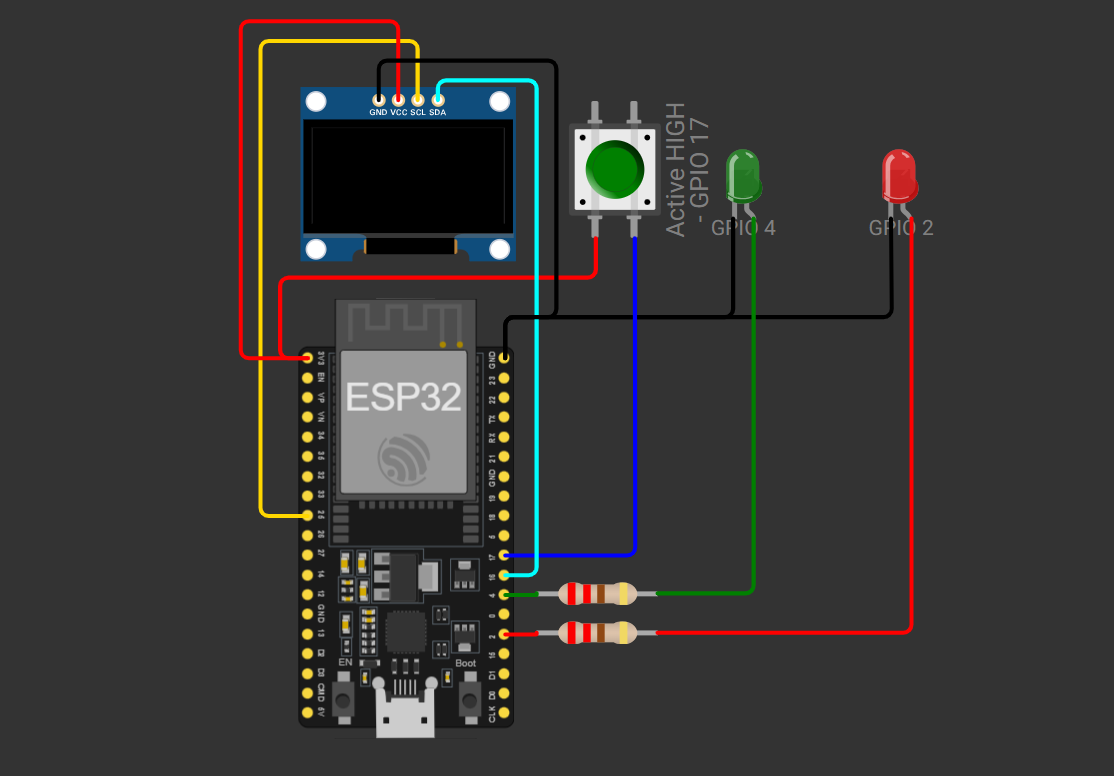
\includegraphics[
    width=\textwidth,
    height=0.66\textheight,
    keepaspectratio
  ]{figures/circuito-wokwi.png}
  \caption{Circuito do projeto no Wokwi: ESP32-DevKitC V4, OLED SSD1306, botão e dois LEDs.}
  \label{fig:circuito}
\end{figure}

A disposição gráfica dos fios pode ser ajustada sem modificar o funcionamento, desde que as extremidades elétricas permaneçam conectadas aos mesmos terminais. O arquivo \texttt{diagram.json} registra tanto as conexões quanto as coordenadas visuais e as instruções de roteamento dos condutores.

\section{Conclusão}

O projeto atende aos requisitos propostos por meio de uma implementação modular e reproduzível. A escolha da ESP32-DevKitC V4 reduz ambiguidades de pinagem, enquanto o uso explícito dos GPIOs preserva a correspondência entre código, documentação e circuito. A comunicação I\textsuperscript{2}C satisfaz adequadamente a necessidade de exibição das mensagens e mantém baixo o número de conexões.

A arquitetura assíncrona permite que o LED vermelho continue piscando enquanto o botão é monitorado e o mostrador é atualizado. O antirrepique por programa elimina a necessidade de filtro externo nesta aplicação, e a atualização do OLED apenas em mudanças de estado reduz processamento e cintilação. Por fim, os testes isolados e progressivos forneceram evidências de funcionamento de cada subsistema antes da integração.

A entrega é complementada por dois meios de acesso: a simulação pública no Wokwi e o repositório versionado no GitHub. Em conjunto, eles possibilitam executar, inspecionar, reproduzir e evoluir o projeto.

\section*{Referências eletrônicas}
\addcontentsline{toc}{section}{Referências eletrônicas}

\begin{itemize}
  \item Projeto no Wokwi: \url{\WokwiURL}
  \item Repositório no GitHub: \url{\GitHubURL}
  \item Guia da ESP32-DevKitC V4: \url{https://docs.espressif.com/projects/esp-dev-kits/en/latest/esp32/esp32-devkitc/user_guide.html}
  \item Referência rápida do MicroPython para ESP32: \url{https://docs.micropython.org/en/latest/esp32/quickref.html}
  \item Biblioteca \texttt{asyncio} do MicroPython: \url{https://docs.micropython.org/en/latest/library/asyncio.html}
  \item Componente SSD1306 do Wokwi: \url{https://docs.wokwi.com/parts/board-ssd1306}
\end{itemize}

\end{document}
